\subsection{Graphical User Interface}

%%Insert some paper citation that indicates user interfaces should be simple and blabla
%The User Interface provides the necessary information about the registered devices in a simple yet effective way;therefore, it is constituted by just two parts

The User Interface is constituted by two parts: the Main Window and the Configuration Dialog.

\subsubsection{Main Window}

The Main Window has two sections: the first allows the connection set-up with the panstamp server while the second displays the overall state of each entity in the network (see Figure ~\ref{java-server-main}). 

To establish a connection, the user has to select the serial port, which the panstamp is attached to, and the corresponding baud-rate. Once the connection is set up, the "connect" button is substituted by a "disconnect" button. The user can disconnect and connect the panstamp at any time. 
% For example if one decides to change the used seria port. 
If the Java server does not detect a device in any of the serial ports, the "connect" button will be unavailable (i.e. grayed out). To prevent the user from constantly restarting the server, we implemented a refresh button, which can be pressed at any time. When a device is finally detected, both options (connect and disconnect) will be available for that device.

The second section of the Main Window shows a table with the overall state of each entity in the network.
Among the data displayed are: the name of the entity's personality, the entity's status and a timestamp.
%explain each possible status (standby, idle, etc)
%explain what the timestamp is for
To reflect new detected entities in the network and changes in the entities' status, the information on the table is periodically updated; the table's refresh rate is configurable. 
%More information in the interface architecture section. %insert link here

\begin{figure}[h!]
 \centering
 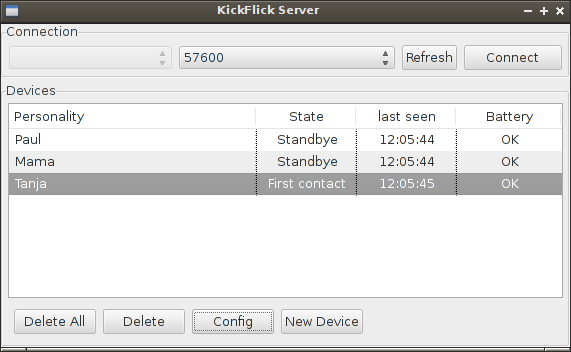
\includegraphics[width= 0.5\textwidth, clip=true  ,keepaspectratio=true]{./pic/java-server-main.png}
 % java-server-main.png: 0x0 pixel, 0dpi, nanxnan cm, bb=
 \caption{Main Window}
 \label{java-server-main}
\end{figure}

If the server detects an entity in the network, the user can select it in the device-table and open a configuration dialog by either pressing the configuration button (located on the bottom of the table) or double clicking on the intended table's item. A configuration dialog will then be opened where this particular device and its personality can be altered.

\subsubsection{Configuration Dialog}

The Configuration Dialog provides all the information about the selected entity's state and allows the configuration of the entity's personality. 

The user can customize a personality or select one among the predefined personalities. But if the user creates a personality and then selects a predefined one, all the changes made so far will be overridden by the predefined personality. 

To cancel all changes, the user has to click the ''close'' button located on the bottom-right corner of the Dialog Window (see Figure ~\ref{fig:java-server-config01}).   

In the Configuration Dialog, the configurable settings of a personality are distributed in 3 different tabs. The tab ''Basic'' (see Figure ~\ref{fig:java-server-config01}) contains the personality's name, the addresses of the two nodes that constitute the entity and a table with all the possible action keys. Only the checked keys will be enabled in the entity; that is, the entity will only react to a certain action key if the latter has a check next to it in the table. Every key can be enabled and disabled by the user. 


\begin{figure}[h!]
 \centering
 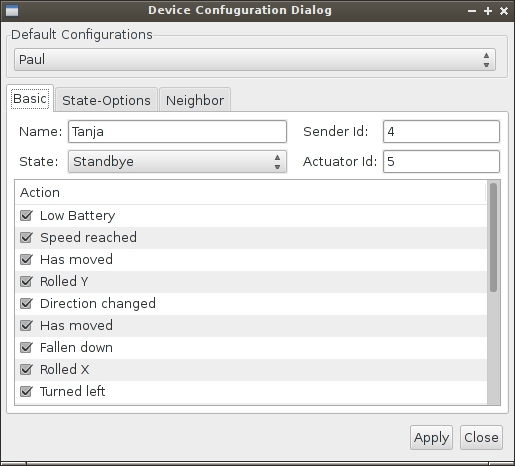
\includegraphics[width= 0.5\textwidth, clip=true  ,keepaspectratio=true]{./pic/java-server-config01.png}
 % java-server-main.png: 0x0 pixel, 0dpi, nanxnan cm, bb=
 \caption{Configuration Dialog, 1st Tab}
 \label{fig:java-server-config01}
\end{figure}

The second tab shows in a checkbox the current state of the device. The state can be changed by the user. Below the checkbox a table with all seperate states of the personality is shown and one can change the pattern and both colors for a particular state. 


\begin{figure}[h!]
 \centering
 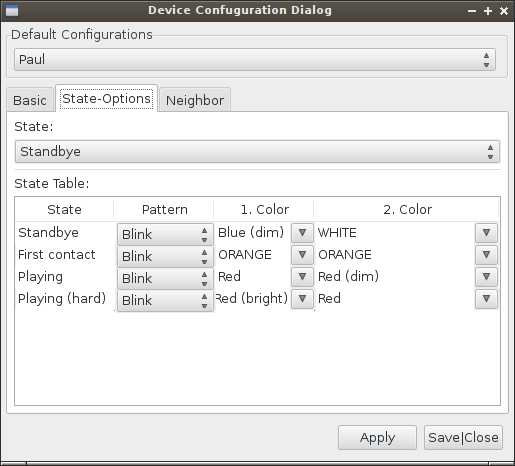
\includegraphics[width= 0.5\textwidth, clip=true  ,keepaspectratio=true]{./pic/java-server-config02.png}
 % java-server-main.png: 0x0 pixel, 0dpi, nanxnan cm, bb=
 \caption{Configuration Dialog, 2nd Tab}
 \label{fig:java-server-config02}
\end{figure}


The third tab displays the actions performed when a neighbor is detected. The table shows every known personality, known by the server at this time. Except for the preset personalities. The preset personalities already know their reaction to the other preset personalities, even if they are yet unknown by the server.
The user can once again configure the pattern and colors of this neighbor reaction. Those settings will then be transmitted to both devices, the one who noticed the neighbor and the neighbor.

After the user finished the configuration and wants to write the new settings to the device, he will need to first press the apply button and then the save and close button to actually writhe the settings. Otherwise if just the save and close button was pressed, no changes will be written and the device remains like before the configuration process.
\begin{figure}[h!]
 \centering
 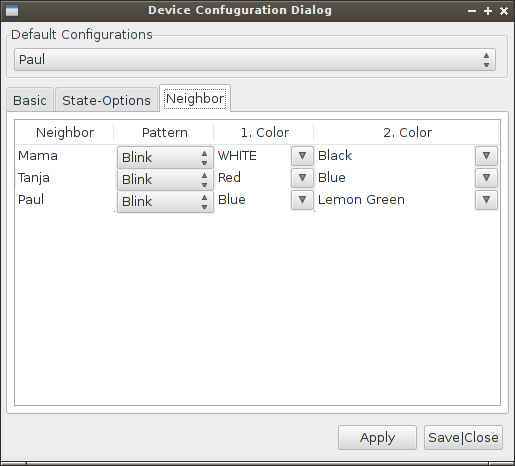
\includegraphics[width= 0.5\textwidth, clip=true  ,keepaspectratio=true]{./pic/java-server-config03.png}
 % java-server-main.png: 0x0 pixel, 0dpi, nanxnan cm, bb=
 \caption{Configuration Dialog, 3rd Tab}
 \label{fig:java-server-config03}
\end{figure}

\subsubsection{Interface Archticture}
The inferface was realised with the swt widget toolkit from eclipse. %insert cite
The main window uses a swt timerevent to periodicly update the device table. Every eventbased action, like button clicks or selection were also realized with the build-in eventlistener structure of the swt toolkit. %insert cite again

When the dialog is opened, the device will be passed as a parameter in the constructor, the dialog will then create the interface and afterwards read the settings of the device. 
The configuration will have no effect on the device at all, except the user says so. All changes will only be written when the apply button is pressed and even then a temporally device will be created to first save all settings in the instance. If the user decides not to use the new settings and wants them to ignored, he then needs to press the windows close button. The close action will pass a null pointer to the main window instance, signaling that no changes were commited.
If, on the other hand, the user wants, after applying, to overwritte the device with the new settings he needs to close the configuration dialog by pressing the save and close button. This will pass a device instance to the main window with all settings and therefor overwrite the previous settings of the device.

The configuration dialog widgets will be filled on the creation of the dialog with all available data, e.g. reaction key names. After the interface is build, the device settings will be set. This happens by for example setting the right selection for a combobox.

The neighbor and state tables are dynamicly created. This way one can decide to add more states and the number of possible neighbors is theoraticly unlimited.


% vim: spell spelllang=en_gb 
